\chapter{Interfejs graficzny użytkownika}
\label{chap:InterfejsGraficznyUżytkownika}
\textit{Autor: Michał Mróz}
\par Aplikacja posiada rozbudowany graficzny interfejs użytkownika, przeznaczony na urządzenia desktopowe. Interfejs dostępny jest w dwóch trybach wizualnych: jasnym i ciemnym, oferując różnorodne efekty kolorystyczne oraz animacje. Dodatkowo aplikacja renderuje dynamicznie pojedyńczy obiekt trójwymiarowy wraz z animacją, co wzbogaca wizualny aspekt interfejsu.

%---
\section{Projektowanie interfejsu graficznego}
\label{sec:ProjektowanieInterfejsuGraficznego}

\emph{Projektowanie interfejsu graficznego \ang{UI Design}}, to proces tworzenia wizualnego środowiska użytkownika przed jego implementacją programistyczną. W ramach naszego projektu inżynierskiego wykorzystałem profesjonalne narzędzie Figma \cite{Figma} do zaprojektowania interfejsu graficznego użytkownika, co pozwoliło usprawnić i ujednolicić dalsze prace związane z implementacją tego interfejsu w kodzie. Projekt graficzny stworzony w \texttt{Figmie} był jedynie przewodnikiem i zaprogramowany interfejs graficzny nie wygląda idealnie tak samo jak jego projekt. 

%---

\subsection{System Projektowania}
\label{sec:SystemProjektowania}

\emph{System projektowania \ang{Design system}} to zestaw standaryzowanych danych i zasobów, które wspólnie definiują wygląd interfejsu graficznego i usprawniają proces projektowania i implementacji. Celem Systemu Projektowania jest zapewnienie spójności wizualnej oraz ułatwienie współpracy między członkami zespołu.
\par
W ramach Systemu Projektowania zdefiniowałem paletę kolorów, rozmiary czcionek i odstępy. Te wartości stałe były konsekwentnie używane przy projektowaniu interfejsu graficznego oraz przy jego implementacji zapewniając spójny wygląd aplikacji.
\begin{figure}[!ht]
    \centering
    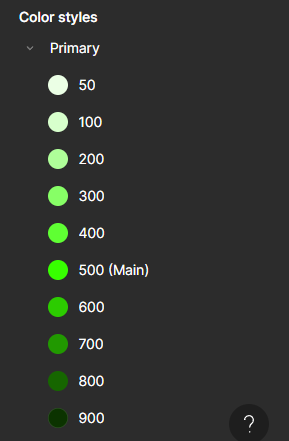
\includegraphics[width=0.5\linewidth, height=7cm]{Images/figma_system_projektowania_1.png}
    \caption{Niektóre kolory z Palety Kolorów}
    \label{fig:enter-label}
\end{figure}

%---

\subsection{Proces projektowania}
\label{sec:ProcesProjektowania}
Po zdefiniowaniu Systemu Projektowania rozpocząłem projektowanie każdej ze stron aplikacji w rozdzielczości 1440x1024 dla urządzeń desktopowych. Wszystkie projekty początkowo powstawały w ciemnej kolorystyce \ang{Dark Mode}, a następnie były kopiowane i dostosowywane do jasnej wersji \ang{Light Mode} pod względem kolorystyki.
\begin{figure}[!ht]
    \centering
    
\includegraphics[width=0.75\linewidth]{Images/figma_projektowanie_1.png}
    \caption{Projekt strony powitalnej w ciemnej kolorystyce}
    \label{fig:enter-label}
\end{figure}
\begin{figure}[!ht]
    \centering
    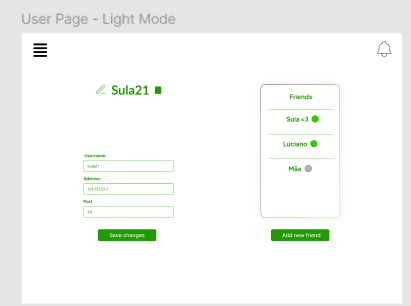
\includegraphics[width=0.75\linewidth]{Images/figma_projektowanie_2.png}
    \caption{Projekt strony profilu użytkownika w jasnej kolorystyce}
    \label{fig:enter-label}
\end{figure}
\begin{figure}[!ht]
    \centering
    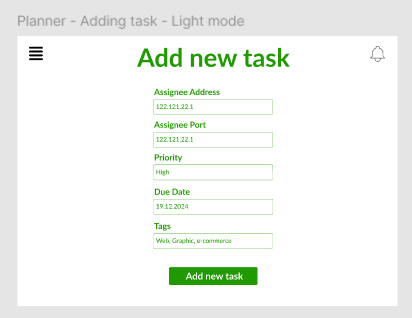
\includegraphics[width=0.75\linewidth]{Images/figma_projektowanie_3.png}
    \caption{Projekt strony dodawania zadania w jasnej kolorystyce}
    \label{fig:enter-label}
\end{figure}
%---

\section{Implementacja Interfejsu Graficznego}
\label{sec:ImplementacjaInterfejsuGraficznego}
Język \texttt{Python} posiada wiele bibliotek do tworzenia interfejsów graficznych, nasz zespół zdecydował się na użycie platformy programistycznej \texttt{QT} w wersji 6 \texttt{(Pyside6)}. Dzięki temu, że ta platforma programistyczna stanowi pakiet w języku \texttt{Python} nasz zespół mógł używać dwóch różnych \texttt{IDE} \ang{Integrated Development Environment} - \texttt{QT Creator} \cite{QT-Creator} i \texttt{Pycharm} \cite{Pycharm}.
Platforma programistyczna \texttt{QT} posiada wiele narzędzi i komponentów umożliwiających tworzenie nie tylko interfejsów graficznych, ale też własnych struktur danych po moduły do pracy z bazami danych, jednakże w naszym projekcie głównie korzystaliśmy z \texttt{Qt do Modelowania (QML)} \ang{Qt Modeling Language} - deklaratywnego języka do tworzenia interfejsów w platformie programistycznej \texttt{QT}. \texttt{QML} oraz \texttt{QT} są wieloplatformowe i działają na urządzeniach desktopowych (\texttt{Windows}, \texttt{Linux}, \texttt{MacOS}) oraz urządzeniach mobilnych i wiele innych.
Dzięki \texttt{QML} możliwe było logiczne rozdzielenie wyglądu od logiki programistycznej, co pozwoliło na zapisanie kodu interfejsu graficznego w odrębnych plikach z rozszerzeniem \texttt{.qml}, ułatwiając tym samym zarządzanie strukturą plików i kodem.

\subsection{Uzasadnienie wyboru Platformy Programistycznej QT}
\label{sec:UzasadnienieWyboruPlatformyProgramistycznejQT}
Przy wyborze technologii do tworzenia interfejsów graficznych w \texttt{Pythonie} mieliśmy do wyboru wiele innych bibliotek, na przykład \texttt{Tkinter}. 
Jednakże w porównaniu do \texttt{Tkinter}, interfejsy w tej bibliotece są przestarzałe wizualnie, a sama biblioteka ta oferuje małe wsparcie dla chociażby efektów wizualnych, animacji, czy responsywności.

Platforma programistyczna \texttt{QT} oraz zawarty w nim \texttt{QML} mają wiele zalet, które nas przekonały do skorzystania z właśnie tej technologii:
\begin{enumerate}
    \item \texttt{QT} jest wieloplatformowy, można w nim tworzyć aplikacje na \texttt{Windowsa}, \texttt{Linuxa}, \texttt{MacOSa} i urządzenia mobilne,
    \item Łatwo jest połączyć logikę strony logicznej z wizualną,
    \item \texttt{QML} umożliwia dodawanie animacji, renderowanie obiektów trójwymiarowych i tworzenie responsywnych interfejsów,
    \item \texttt{QT} posiada ogromną dokumentację i ma szeroką społeczność użytkowników,
    \item \texttt{QT} zapewnia rozdzielenie kodu strony wizualnej \texttt{(QML)} od części logicznej \texttt{(Python)}
\end{enumerate}

\subsection{Podstawy Języka Modelowania QT} 
\label{sec:PodstawyJezykaModelowaniaQT}
\emph{Qt Modeling Language} to język deklaratywny, podobny do CSS i HTML, wchodzący w skład modułu \texttt{QtQuick} platformy programistycznej \texttt{Qt}. Aby zacząć używać \texttt{QML}, należy stworzyć plik \texttt{.qml}, w którym przykładowo możemy zawrzeć:

\begin{lstlisting}[language=QML, caption={Przykładowy kod QML}]
import QtQuick 2.0

Rectangle {
    id: kwadrat
    width: 100
    height: 100
    color: "red"
}
\end{lstlisting}
\listings{Przykładowy kod QML}
Kod ten tworzy kwadrat 100x100 w kolorze czerwonym. Struktura w \texttt{QML} jest hierarchiczna. Oznacza to, że wewnątrz komponentu \texttt{Rectangle} moglibyśmy dodać kolejny obiekt, który byłby tworzony względem rodzica - \texttt{Rectangle}.

Dodatkowo \texttt{QML} umożliwia pisanie języka \texttt{Javascript} w odpowiednich polach,
na przykład do kodu w kwadracie można dodać:

\begin{lstlisting}[language=QML, caption={Przykładowy Javascript}]
Component.onCompleted: {
    console.log(kwadrat.width);
}
\end{lstlisting}
\listings{Przykładowy Javascript}
który wypisze w konsoli szerokość kwadratu.


\subsection{Zaimplementowane istotne mechanizmy}
\label{sec:ZaimplementowaneIstotneMechanizmy}

\subsubsection{Struktura Interfejsu}
\label{sec:Struktura Interfejsu}
W naszym projekcie każdy osobny plik \texttt{.qml} stanowi osobną stronę interfejsu lub
definicję niestandardowego komponentu. Niestandardowe komponenty są zawarte
w osobnych folderach: 
\begin{lstlisting}
"app_style", "gui_components", "small_gui_components"
\end{lstlisting}

Omówię najpierw aspekt niestandardowych komponentów. W \texttt{QML} można tworzyć własne klasy komponentów.

\begin{lstlisting}[language=QML, caption={Przykładowa klasa w MyRectangle.qml}]
Rectangle {
    id: rectangle
    color: "blue"
    width: 100
    height: 100
}
\end{lstlisting}
\listings{Przykładowa klasa w MyRectangle.qml}
Zaimportowanie tego w innym pliku \texttt{(Page1.qml)} umożliwi stworzenie
wielu instancji klasy \texttt{MyRectangle}:

\begin{lstlisting}[language=QML, caption={Przykładowe użycie klasy MyRectangle}]
MyRectangle {} //niebieski kwadrat 100x100
MyRectangle {color: "red"} //czerwony kwadrat 100x100
\end{lstlisting}
\listings{Przykładowe użycie klasy MyRectangle}
Pozwala to na uniknięcie redundancji w kodzie, gdy trzeba tworzyć
wiele obiektów, różniących się, tylko niektórymi atrybutami.

W naszym projekcie jest to wykorzystywane przy tworzeniu list, chociażby
użytkowników albo własnych przycisków, których w interfejsie jest pełno i dzięki definiowaniu ich w jednej klasie, wyglądają podobnie i upraszczają kod.

Reszta plików \texttt{.qml} stanowi osobne strony interfejsu. 
Tworząc komponent StackView oraz używając:
\begin{lstlisting}[language=QML, caption={Ładowanie nowej strony}]
stackView.push("nazwa_pliku.qml");
\end{lstlisting}
\listings{Ładowanie nowej strony}
można w bardzo prosty sposób załadować nową stronę.
Taki podział (strona - plik) sprawia, że struktura interfejsu jest bardziej
uporządkowana oraz logiczna i upraszcza to pracę z kodem.

\subsubsection{Implementacja Systemu Projektowania}
\label{sec:ImplementacjaSystemuProjektowania}
System Projektowania z części Projektowania Interfejsu Graficznego zakłada użycie stałych wartości kolorów, odstępów oraz wielkości czcionek.

Nasz projekt implementuje to w folderze \texttt{app\_style} w trzech plikach \texttt{QML}:

\begin{enumerate}
    \item ColorPalette.qml - Definiujący zestaw stałych kolorów
    \item FontStyle.qml - Definiujący czcionkę oraz różne rozmiary
    \item SpacingObjects.qml - Definiujący wartości odstępów między elementami w interfejsie
\end{enumerate}

Każdy z nich zawiera analogiczną logikę, więc omówię na przykładzie klasy \texttt{ColorPalette}:

W kodzie \texttt{QML} definiujemy zmienne stałe w sposób poniższy.

\begin{lstlisting}[language=QML, caption={ColorPalette.qml}]
import QtQuick 2.15

QtObject {
    readonly property color primary50: "#EBFFE5"
    readonly property color primary100: "#D7FFCC"
    ...

    readonly property color secondary50: "#FEE5FF"
    readonly property color secondary100: "#FDCCFF"
    ...
\end{lstlisting}
\listings{ColorPalette.qml}

Następnie w bardzo prosty sposób możemy używać tych stałych wartości w każdym miejscu w kodzie:
\begin{lstlisting}[language=QML, caption={Przykładowe użycie palety kolorów}]
import "../app_style"

//User (Peer) List Class Blueprint
Rectangle {
ColorPalette { id: colorPalette }
...

    property string list_color: settings.light_mode ? colorPalette.background50 : colorPalette.background800
    ...
\end{lstlisting}  
\listings{Przykładowe użycie palety kolorów}

\subsubsection{Komunikacja ze Stroną Logiczną}
\label{sec:KomunikacjaZeStronaLogiczna}
Komunikacja ze stroną logiczną aplikacji w platformie programistycznej \texttt{QT} odbywa się za pomocą \texttt{Sygnałów} \ang{Signal} i \texttt{Gniazd} \ang{Slot}. Ten sam mechanizm istnieje również, gdy używamy \texttt{QT} wraz z językiem \texttt{C++}, jednakże składnia jest inna. 

\texttt{Sygnał} to obiekt, który jak nazwa wskazuje ma za zadanie wysłanie \texttt{Sygnału},
dokonuje się tego przy pomocy metody \texttt{.emit()}.

\texttt{Slot} to specjalna funkcja, którą należy połączyć z wybranym, uprzednio stworzonym \texttt{Sygnałem}.

Po wysłaniu sygnału zostaje wywołany podłączony do niego \texttt{Slot}. Dodatkowo w metodzie \texttt{.emit()} można przesyłać argumenty.

Jeżeli chcemy osiągnać komunikację między stroną logiczną, a stroną wizualną to musimy:

\begin{enumerate}
    \item Zdefiniować sygnał w klasie w \texttt{Pythonie}, który potem należy podłączyć do zdefiniowanej w \texttt{QML} za pomocą \texttt{JavaScript} funkcji \texttt{(Slot)} i następnie wywołać \texttt{.emit()} z poziomu \texttt{Pythona} dla tego sygnału. To umożliwi wywołanie funkcji zawartej w \texttt{QML} za pomocą kodu w Pythonie.
    \item Możemy też pójść w drugą stronę – jeśli chcemy wywołać coś ze strony logicznej przy użyciu kodu \texttt{QML}, wtedy należy stworzyć \texttt{Slot} w klasie w \texttt{Pythonie}, gdzie kod \texttt{QML} staje się \texttt{Sygnałem}.
\end{enumerate}

Istotnym aspektem jest to, że samo przekazanie wartości do strony wizualnej jest operacją prostą, można tego dokonać jednorazowo przy inicjalnym ładowaniu interfejsu, o czym za chwilę, jednakże mechanizm sygnałów i slotów umożliwia dynamiczne przekazywanie informacji między stroną wizualną a logiczną.

Na przykład jeśli dodamy kogoś do znajomych, to w stronie logicznej w funkcji która odpowiada za dodanie użytkownika do znajomych możemy wywołać \texttt{.emit()} i dynamicznie obsłużyć tą zmianę w stronie wizualnej.

Teraz pokazując kod z naszego projektu omówię na przykładzie jak wykorzystaliśmy ten mechanizm.

Przykładowo, żeby dynamicznie obsłużyć zmianę znajomych w naszym programie, w stronie logicznej, wykorzystujemy atrybut \texttt{self.peers} który w klasie \texttt{User} zawiera tablicę innych obiektów tego typu, ostatecznie przekazujemy je do strony wizualnej i wypisujemy na ekranie.

Tworzymy sygnał w klasie \texttt{User}:
\begin{lstlisting}[language=Python, caption={Sygnał User}]
class User(QObject):
    peersChanged = Signal()
\end{lstlisting}   
\listings{Sygnał User}

Definiujemy tablicę peers jako \texttt{Property}:
\begin{lstlisting}[language=Python, caption={Peers Property}]
@Property("QVariantList", notify=peersChanged)
    def peers(self):
        return self._peers
\end{lstlisting}
\listings{Peers Property}

W pliku \texttt{main.py} przed inicjalnym załadowaniem interfejsu możemy przekazać uprzednio stworzony pojedyńczy obiekt \texttt{User}, gdzie u nas jest to obecny użytkownik programu. Teraz w \texttt{QML} możemy używać metod i atrybutów tej klasy dla tego obiektu.

\begin{lstlisting}[language=Python, caption={Przekazanie inicjalnego obiektu}]
engine.rootContext().setContextProperty("user", user)
\end{lstlisting}
\listings{Przekazanie inicjalnego obiektu}

Teraz w klasie \texttt{FriendList}, po załadowaniu komponentu należy podłączyć sygnał \texttt{peersChanged} z funkcją w języku \texttt{JavaScript}, która przetwarza dane znajomych z obiektu \texttt{User}.

\begin{lstlisting}[language=Python, caption={Podłączenie sygnału do slota w QML}]
Component.onCompleted: {
        user.peersChanged.connect(updateUserModel);
}
\end{lstlisting}
\listings{Podłączenie sygnału do slota w QML}
Teraz każdy zapis \texttt{peersChanged.emit()} w \texttt{Pythonie} spowoduje wywołanie funkcji \texttt{updateUserModel()}, która u nas w projekcie, wygląda tak:

\begin{lstlisting}[language=Python, caption={Slot w QML obsługujący wyświetlanie zmienionej listy znajomych}]
function updateUserModel() {
    userModel.clear();

    // Iterate over peers array passed from Python
    for (let i = 0; i < user.peers.length; i++) {
        ...
        ...
        userModel.append({
            nickname: user.peers[i].nickname,
            host: host,
            port: port,
            active: user.peers[i].active,
            isInGroup: isInGroup,
            isSelected: isSelected,
            activeColor: activeColor
        });
    }
}
\end{lstlisting}
\listings{Slot w QML obsługujący wyświetlanie zmienionej listy znajomych}
Dla uproszczenia można założyć, że komponent \texttt{userModel} to po prostu lista znajomych.
\par
W ten sposób możemy dynamicznie aktualizować wyświetlane dane w stronie wizualnej za każdym razem, gdy lista znajomych \texttt{(self.peers)} ulegnie zmianie.

Na przykład funkcja odpowiadająca za usunięcie znajomego, która jest \texttt{Slotem} - wywoływana jest z poziomu strony wizualnej po kliknięciu przycisku, a strona logiczna informuje stronę wizualną o usunięciu znajomego za pomocą metody \texttt{.emit()}, a ten następnie przetwarza tą zmianę i wyświetla na ekranie:
\begin{lstlisting}[language=Python, caption={Przykładowe użycie sygnału dla listy znajomych}]
@Slot(str, int)
def removeFromPeers(self, host, port):
    for peer in self.peers:
        if peer.host == host and peer.port == port:
            self.peers.remove(peer)
            self.peersChanged.emit()
            break
\end{lstlisting}
\listings{Przykładowe użycie sygnału dla listy znajomych}

\subsubsection{Renderowanie Obiektu Trójwymiarowego}
\label{sec:RenderowanieObiektuTrójwymiarowego}
Nasza aplikacja renderuje jeden obiekt trójwymiarowy, istotne jest to, że korzystamy z dynamicznego renderera obiektów trójwymiarowych zamiast na przykład prostych ruchomych obrazków.
\texttt{QT} umożliwia renderowanie obiektów trójwymiarowych w \texttt{QML}, przy użyciu modułu \texttt{Qt3D} \cite{QT3D}, który w naszym projekcie umożliwia renderowanie trójwymiarowego kształtu i jego animacje (obrót do okoła osi).

% responsywność interfejsu i skalowanie komponentów
\subsubsection{Responsywność interfejsu}
\label{sec:ResponsywnośćInterfejsu}
Aplikacja zapewnia responsywność interfejsu przy skalowaniu okna aplikacji. Elementy posiadają zdefiniowaną szerokość oraz wysokość, których wartości nie są stałą liczbą, lecz stanowią procentową wartość rozmiarów okna aplikacji.
\begin{lstlisting}[language=QML, caption={Przykładowy element o szerokości 1/6}]
TaskElementInfo {
    rect_width: parent.width / 6
\end{lstlisting}
\listings{Przykładowy element o szerokości 1/6}
Dodatkowo uzależniliśmy wielkości czcionek oraz odstępów od wielkości okna aplikacji definiując odpowiednie funkcje skalujące, które są używane wielokrotnie w całym kodzie strony wizualnej.
\begin{lstlisting}[language=QML, caption={Funkcja skalująca odstępy}]
readonly property var base_x: 1280.0
readonly property var base_y: 720.0
    
//axis boolean - 0 is X, 1 is Y
function preserveSpacingProportion(spacing, width, height, axis) {
   if(!axis) return width / base_x * spacing;
   else return height / base_y * spacing;
}
\end{lstlisting}
\listings{Funkcja skalująca odstępy}

\subsection{Pomoce naukowe związane z platformą programistyczną QT i językiem modelowania QT}
\label{sec:PomoceNaukoweQML}
Przy pracy z platformą programistyczną \texttt{QT} oraz \texttt{QML} korzystaliśmy z ogromnej oficjalnej dokumentacji: 
\par
Dokumentacja \texttt{QT} \cite{DokumentacjaQT}
\par
Dokumentacja \texttt{QML} \cite{DokumentacjaQML}
\par
Dokumentacja \texttt{QT for Python} \cite{DokumentacjaQtForPython}.
\par
Korzystaliśmy również z poradnika na youtubie:
Poradnik: \cite{PoradnikQMLYoutube}